\chapter{Triangles, Angles, and Parallels}


\section{Angles}
In the following recommended videos, the narrator talks about
lines, line segments, and rays. When mathematicians talk about
\emph{lines}\index{lines}, they mean a straight line that goes forever in two 
directions. If you pick any two points on that line, the space between 
them is a \emph{line segment}\index{line segment}. If you take any line, pick 
a point on it, and discard all the points on one side of the point, that 
is a \emph{ray}\index{ray}. All three have no width.

\begin{center}
\begin{tikzpicture}[scale=1.5]
  \coordinate (a) at (-0.3, -0.6);
  \coordinate (d) at (1.3, 2.6);
  \draw [<->](a)--node [right]{"Line"}(d);
\end{tikzpicture}
\hspace{10mm}
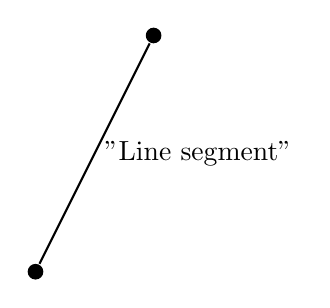
\begin{tikzpicture}[scale=1.5]
  \coordinate [circle, fill, inner sep=2pt] (b) at (0,0) ;
  \coordinate [circle, fill, inner sep=2pt] (c) at (1, 2) ;
  \draw (b)--node [right]{"Line segment"}(c);
\end{tikzpicture}
\hspace{6mm}
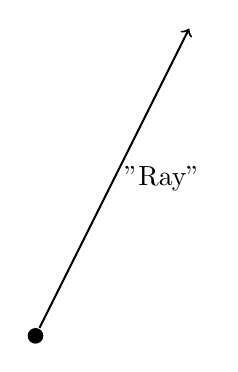
\begin{tikzpicture}[scale=1.5]
  \coordinate [circle, fill, inner sep=2pt] (b) at (0,0) ;
  \coordinate (d) at (1.3, 2.6);
  \coordinate (lab) at (0.8, 1.0);
  \draw [->](b)--node[right] {"Ray"} (d)  ;
\end{tikzpicture}
\end{center}



Watch the following videos from Khan Academy:
\begin{itemize}
\item Introduction to angles: \url{https://youtu.be/H-de6Tkxej8}
\item Measuring angles in degrees: \url{https://youtu.be/92aLiyeQj0w} 
\end{itemize}

When two lines cross, they form four \index{angle}angles:

\begin{center}
\begin{tikzpicture}[scale=3]
  \coordinate (a) at (0, 1.5);
  \coordinate (b) at (1.6, 2);
  \coordinate (c) at (1.6, 1.5);
  \coordinate (d) at (0, 1);
  \coordinate [circle, fill, inner sep=1pt](e) at (0.8, 1.5) ;
  \draw [->](e)--(a) node[left] {$A$}  ;
  \draw [->](e)--(b) node[right] {$B$}  ;
  \draw [->](e)--(c) node[right] {$C$}  ;
  \draw [->](e)node[above]{$E$}--(d) node[left] {D} ;
  \pic [draw, <->, "$\scriptstyle  \angle AEB$ ", angle radius = 0.8cm, 
  angle eccentricity=1.3] {angle = b--e--a};
  \pic [draw, <->, "$\scriptstyle  \angle BEC$ ", angle radius = 1.1cm, 
  angle eccentricity = 1.5] {angle = c--e--b};
  \pic [draw, <->, "$\scriptstyle  \angle CED$ ", angle radius = 0.8cm, 
  angle eccentricity=1.3] {angle = d--e--c};
  \pic [draw, <->, "$\scriptstyle  \angle DEA$ ", angle radius = 1.1cm, 
  angle eccentricity=1.5] {angle = a--e--d};
\end{tikzpicture}
\end{center}


What do we know about those angles? (Note that $m \angle$ means "the measure of angle")
\begin{itemize}
\item The sum of any two adjacent angles adds to be $180^\circ$ So, for 
example, $m \angle AEB + m \angle BEC = 180^\circ$. We use the phrase ``adds to 
be $180^{\circ}$'' so often that we have a special word for it: 
\emph{supplementary}.\index{supplementary angles}
\item The sum of all four angles is $360^\circ$.
\item Angles opposite each other are equal. So, for example, $m \angle AEB = m 
\angle CED$.
\item Angles that sit side by side along a straight line add up to $180^\circ$. For example, the angles on one side of $\overline{AC}$ add up to $180^\circ$.
\end{itemize}

In a diagram, to indicate that two angles are equal we often put hash marks in 
the angle:

\begin{center}
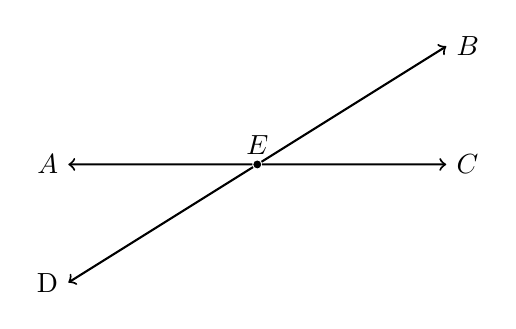
\begin{tikzpicture}[scale=3]
  \coordinate (a) at (0, 1.5);
  \coordinate (b) at (1.6, 2);
  \coordinate (c) at (1.6, 1.5);
  \coordinate (d) at (0, 1);
  \coordinate [circle, fill, inner sep=1pt](e) at (0.8, 1.5) ;
  \draw [->](e)--(a) node[left] {$A$}  ;
  \draw [->](e)--(b) node[right] {$B$}  ;
  \draw [->](e)--(c) node[right] {$C$}  ;
  \draw [->](e)node[above]{$E$}--(d) node[left] {D} ;
  \tkzMarkAngle[size = 0.2cm,mark = |](b,e,a)
  \tkzMarkAngle[size = 0.3cm,mark = ||](c,e,b)
  \tkzMarkAngle[size = 0.2cm,mark = |](d,e,c)
  \tkzMarkAngle[size = 0.3cm,mark = ||](a,e,d)
\end{tikzpicture}
\end{center}


Here, the two angles with a single hash mark are equal, and the two angles with 
double hash marks are equal.

When two lines are perpendicular, the angle between them is $90^\circ$, and we 
say they meet at a \emph{right angle}\index{right angle}. When drawing diagrams, we indicate right
angles with an elbow:

\begin{center}
\begin{tikzpicture}[scale=1.5]
  \coordinate (a) at (0, 1.5);
  \coordinate (b) at (0, 0);
  \coordinate (c) at (1.5, 0);
  \draw [->](b)--(a)  ;
  \draw [->](b)--(c)  ;
  \pic [draw,thick,angle eccentricity=.5]{right angle = a--b--c};
\end{tikzpicture}
\end{center}

 
When an angle is less than $90^\circ$, it is said to be
\emph{acute}\index{acute angle}. When an angle is more than $90^\circ$, it is said to be
\emph{obtuse}\index{obtuse angle}.

Just as two angles which add up to $180^\circ$ are referred to as supplementary angles,
two (or more) angles which add up to $90^\circ$ are \emph{complementary} angles.\index{complementary angles} For example, two $45^\circ$ angles are complementary, as well as $30^\circ$ and $60^\circ$. If an angle is $65^\circ$, we say that its \emph{complement} is $90^\circ-65^\circ=25^\circ$.
% Add: Complementary Angles

\begin{center}
\begin{tikzpicture}[scale=3]
  \coordinate (a) at (0.4, 0.6);
  \coordinate (b) at (0, 0);
  \coordinate (c) at (0.9, 0);
  \draw [->](b)--(a)  ;
  \draw [->](b)--(c)  ;
  \pic [draw, <->, "acute", angle radius = 1cm, angle eccentricity=1.5] {
  angle = c--b--a};
  \end{tikzpicture}
\hspace{2cm}
\begin{tikzpicture}[scale=3]
  \coordinate (a) at (1, 0.6);
  \coordinate (b) at (0.5, 0);
  \coordinate (c) at (0, 0);
  \draw [->](b)--(a)  ;
  \draw [->](b)--(c)  ;
  \pic [draw, <->, "obtuse", angle radius = 0.6cm, angle eccentricity=1.5] {
  angle = a--b--c};
\end{tikzpicture}
\end{center}


If two lines are parallel (never intersecting lines with points all the same distance apart), line segments that intersect both lines (\index{transversal}transversals) form the
same angles with each line:
%parallel is not introduced until chapter 5
\begin{center}
\begin{tikzpicture}[scale=3]
  \coordinate (a) at (0, 1);
  \coordinate [circle, fill, inner sep=1pt](b) at (1.5, 1.5);
  \coordinate (c) at (1.5, 1);
  \coordinate (d) at (0.5, 0.5);
  \coordinate (e) at (1, 1);
  \coordinate (f) at (0, 0.5);
  \coordinate (g) at (1.5, 0.5);
  \coordinate [circle, fill, inner sep=1pt](h) at (0, 0);
  \draw [->](e)--(a);
  \draw [-](e)--(b);
  \draw [->](e)--(c);
  \draw [-](e)--(d);
   \draw [->](d)--(f);
  \draw [->](d)--(g);
  \draw [-](d)--(h);
  \tkzMarkAngle[size = 0.15cm,mark = |](b,e,a)
  \tkzMarkAngle[size = 0.2cm,mark = ||](c,e,b)
  \tkzMarkAngle[size = 0.15cm,mark = |](d,e,c)
  \tkzMarkAngle[size = 0.2cm,mark = ||](a,e,d)
  
   \tkzMarkAngle[size = 0.15cm,mark = |](e,d,f)
  \tkzMarkAngle[size = 0.2cm,mark = ||](g,d,e)
  \tkzMarkAngle[size = 0.15cm,mark = |](h,d,g)
  \tkzMarkAngle[size = 0.2cm,mark = ||](f,d,h)
\end{tikzpicture}
\end{center}


\subsection{Radians}
As you have seen above, angles can be measured in \index{degrees}degrees. Just like you can 
measure length in more than one unit (inches, meters, etc.), there is more 
than one unit to measure angles in. Angles can also be measured in \textit{
radians}\index{radians}. Radians are unitless (that is, you do not have to put 
a letter after the number) and there are $\pi$ radians across a straight line. 
On diagrams and equations, unknown angles in radians are usually represented with the greek letter $\theta$.
This means $180^\circ$ is the same as $\pi$ radians. 
Radians come from comparing the length of an arc to the radius of a circle--which we will explore in a future chapter.

Generally, you can use the following formula for your conversions:
$${\displaystyle {\text{angle in degrees}}={\text{angle in radians}}\cdot {\frac {180^{\circ }}{\pi }}}$$

\textbf{Example}: An angle is measured to be $\frac{\pi}{2}$ radians. What is 
the angle in degrees?

\textbf{Solution}: Since we know that $\pi$ radians is the same as $180^\circ$,
we can set up the unit conversion:
$$\frac{\pi}{2} \cdot \frac{180^\circ}{\pi} = 90^\circ$$

Therefore, a $\frac{\pi}{2}$ angle is $90^\circ$. 


\begin{Exercise}[label = radians]
Convert the following angles from degrees to radians, or from radians to degrees. 
\begin{enumerate}
\item $360^\circ$
\item $\frac{\pi}{3}$
\item $225^\circ$
\item $\frac{3\pi}{4}$
\item $30^\circ$
\item $45^\circ$
\end{enumerate}
\end{Exercise}

\begin{Answer}[ref = radians]
\begin{enumerate}
\item $2\pi$
\item $60^\circ$
\item $\frac{5\pi}{4}$
\item $135^\circ$
\item $\frac{\pi}{6}$
\item $\frac{\pi}{4}$
\end{enumerate}
\end{Answer}


\section{Introduction to Triangles}
Connecting any three points with three line segments will get you a
triangle. Here is the triangle $ABC$, which was created by connecting three points $A$, $B$, and $C$:\index{triangle}

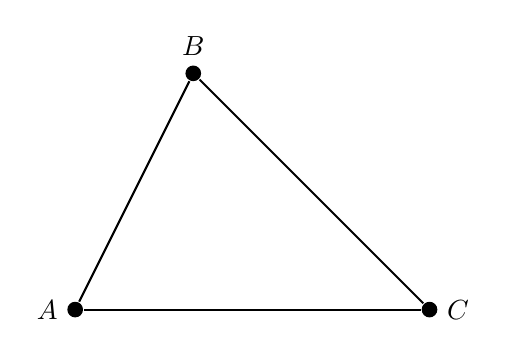
\begin{tikzpicture}[scale=1.5]
  \coordinate [circle, fill, inner sep=2pt] (a) at (0,0) ;
  \coordinate [circle, fill, inner sep=2pt] (b) at (1, 2) ;
  \coordinate [circle, fill, inner sep=2pt] (c) at (3,0) ;
  \draw (a)--(b) node [outer sep=3pt, above]{$B$};
  \draw (b)--(c) node[outer sep=3pt, right]{$C$};
  \draw (c)--(a) node[outer sep=3pt, left]{$A$};
\end{tikzpicture}

\subsection{Equilateral, Isosceles, and Scalene Triangles}
We talk a great deal about the length of the sides of triangles. If all three sides of the triangle are the same length, we say it is an \emph{equilateral triangle}:\index{equilateral triangle}
\begin{center}
  \begin{tikzpicture}[scale=1.5]
  \coordinate [circle, fill, inner sep=2pt] (a) at (0,0) ;
  \coordinate [circle, fill, inner sep=2pt] (b) at (1.5, 2.6) ;
  \coordinate [circle, fill, inner sep=2pt] (c) at (3,0) ;
  \draw (a)--(b) node [outer sep=3pt, above]{$B$};
  \draw (b)--(c) node[outer sep=3pt, right]{$C$};
  \draw (c)--(a) node[outer sep=3pt, left]{$A$};
  \tkzMarkSegment[pos=.5,mark=||](a,b)
  \tkzMarkSegment[pos=.5,mark=||](b,c)
  \tkzMarkSegment[pos=.5,mark=||](c,a)
\end{tikzpicture}
\end{center}

If only two sides of the triangle are the same length, we say it is an \emph{isosceles triangle}:\index{isosceles triangle}
\begin{center}
\begin{tikzpicture}[scale=1.3]
  \coordinate [circle, fill, inner sep=2pt] (a) at (0,0) ;
  \coordinate [circle, fill, inner sep=2pt] (b) at (1.5, 4) ;
  \coordinate [circle, fill, inner sep=2pt] (c) at (3,0) ;
  \draw (a)--(b) node [outer sep=3pt, above]{$B$};
  \draw (b)--(c) node[outer sep=3pt, right]{$C$};
  \draw (c)--(a) node[outer sep=3pt, left]{$A$};
  \tkzMarkSegment[pos=.5,mark=||](a,b)
  \tkzMarkSegment[pos=.5,mark=||](c,b)
\end{tikzpicture}
\end{center}
When all three sides of a triangle are different, the triangle is referred to as \emph{scalene}. \index{Scalene Triangle}This consequently means all angle measures are different as well.
\begin{center}
  
\begin{tikzpicture}[scale=1.3]
  \coordinate [circle, fill, inner sep=2pt] (a) at (0,0) ;
  \coordinate [circle, fill, inner sep=2pt] (b) at (1.5, 4) ;
  \coordinate [circle, fill, inner sep=2pt] (c) at (3,5) ;
  \draw (a)--(b) node [outer sep=3pt, above]{$B$};
  \draw (b)--(c) node[outer sep=3pt, right]{$C$};
  \draw (c)--(a) node[outer sep=3pt, left]{$A$};
\end{tikzpicture}
\end{center}


The shortest distance between two points is always the straight line
between them. This means you can be certain that the length of one side
will \emph{always} be less than the sum of the lengths of the
remaining two sides. This is known as the \emph{triangle inequality}.\index{triangle inequality}

For example, in this diagram, $c$ must be less than $a + b$.

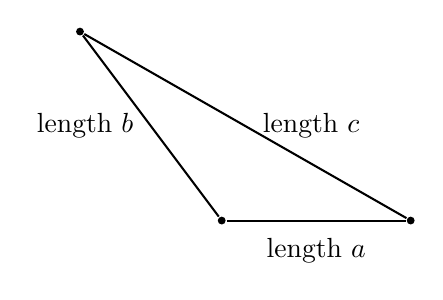
\begin{tikzpicture}[scale=1.2]
  \coordinate [circle, fill, inner sep=1pt] (a) at (1.5,0) ;
  \coordinate [circle, fill, inner sep=1pt] (b) at (0,2) ;
  \coordinate [circle, fill, inner sep=1pt] (c) at (3.5,0) ;
  \draw (a)--node[outer sep=3pt, left]{length $b$}(b) ;
  \draw (b)--node[outer sep=3pt, right]{length $c$}(c) ;
  \draw (c)--node[outer sep=3pt, below]{length $a$}(a) ;
\end{tikzpicture}

\subsection{Interior Angles of a Triangle}

We also talk a lot about the \index{interior angles}interior angles of a triangle:

\begin{tikzpicture}[scale=2]
  \coordinate [circle, fill, inner sep=2pt] (a) at (0,0) ;
  \coordinate [circle, fill, inner sep=2pt] (b) at (1, 2) ;
  \coordinate [circle, fill, inner sep=2pt] (c) at (3,0) ;
  \draw (a)--(b) node [outer sep=3pt, above]{$B$};
  \draw (b)--(c) node[outer sep=3pt, right]{$C$};
  \draw (c)--(a) node[outer sep=3pt, left]{$A$};
  \pic [draw, <->, "$a$", angle eccentricity=1.5] {angle = c--a--b};
  \pic [draw, <->, "$b$", angle eccentricity=1.5] {angle = a--b--c};
  \pic [draw, <->, "$c$", angle eccentricity=1.5] {angle = b--c--a};
\end{tikzpicture}

A triangle where one of the interior angles is a right angle is said to be a \emph{right triangle}:\index{right triangle} The side opposite the right angle is the longest side, referred to as the \index{hypotenuse}hypotenuse.

\begin{tikzpicture}[scale=1.2]
  \coordinate [circle, fill, inner sep=2pt] (a) at (0,0) ;
  \coordinate [circle, fill, inner sep=2pt] (b) at (0,4) ;
  \coordinate [circle, fill, inner sep=2pt] (c) at (3,0) ;
  \draw (a)--(b) node [outer sep=3pt, above]{$B$};
  \draw (b)--(c) node[outer sep=3pt, right]{$C$};
  \draw (c)--(a) node[outer sep=3pt, left]{$A$};
  \pic [draw,angle eccentricity=1.5] {right angle = c--a--b};
\end{tikzpicture}

If a triangle has an obtuse interior angle, it is said to be an \emph{obtuse triangle}:\index{obtuse triangle}

\begin{tikzpicture}[scale=1.2]
  \coordinate [circle, fill, inner sep=2pt] (a) at (1.5,0) ;
  \coordinate [circle, fill, inner sep=2pt] (b) at (0,2) ;
  \coordinate [circle, fill, inner sep=2pt] (c) at (3.5,0) ;
  \draw (a)--(b) node [outer sep=3pt, above]{$B$};
  \draw (b)--(c) node[outer sep=3pt, right]{$C$};
  \draw (c)--(a) node[outer sep=3pt, left]{$A$};
  \pic [draw, <->, "obtuse", angle eccentricity=1.7] {angle = c--a--b};
\end{tikzpicture}

If all three interior angles of a triangle are less than $90^\circ$, it is said to be an \emph{acute triangle}.\index{acute triangle}

The measures of the interior angles of a triangle always add up to
$180^\circ$. For example, if we know that a triangle has interior
angles of $37^\circ$ and $56^\circ$, we know that the third
interior angle is $87^\circ$.

\begin{Exercise}[title={Missing Angle}, label=missing_angle]
One interior angle of a triangle is $92^\circ$. The second angle is $42^\circ$. What is the measure of the third interior angle?
\end{Exercise}
\begin{Answer}[ref=missing_angle]
$180^\circ - (92^\circ + 42^\circ) = 46^\circ$
\end{Answer}

How can you know that the sum of the interior angles is $180^\circ$?
Imagine that you started on the edge of a triangle and walked all the
way around to where you started, going counter-clockwise. You would turn left three times:

\begin{tikzpicture}[scale=1.7]
  \coordinate [circle, fill, inner sep=2pt] (a) at (1.5,0) ;  
   \node at (a) [outer sep=3pt, left]{$A$};
  \coordinate [circle, fill, inner sep=2pt] (b) at (0.5,2) ;
  \node at (b) [outer sep=3pt, above]{$B$} ;
  \coordinate [circle, fill, inner sep=2pt] (c) at (3.5,0) ;
    \node at (c)[outer sep=3pt, below]{$C$};
    
    \coordinate [circle, fill, inner sep=2pt](start) at (2.75,0);
    \node at (start)[outer sep=3pt, below]{Start};

   \coordinate (aa) at (1.75,-0.5) ;  
  \coordinate (bb) at (-0.25,2.5) ;
  \coordinate (cc) at (4.2,0) ;
  \draw [->](a)--(cc);
  \draw [->](b)--(aa);
  \draw [->](c)--(bb);
  \pic [draw, ->, "$T_C$", angle eccentricity=1.7] {angle = cc--c--b};
  \pic [draw, ->, "$T_B$", angle eccentricity=2] {angle = bb--b--a};
  \pic [draw, ->, "$T_A$", angle eccentricity=2] {angle = aa--a--c};
\end{tikzpicture}

After these three turns, you would be facing the same direction that
you started in. Thus, $T_A + T_B + T_C = 360^\circ$. The
measures of the interior angles are $a$, $b$, and $c$. Notice that $a$ and
$T_A$ are supplementary. So we know that:
\begin{itemize}
\item $T_A = 180 - a$
\item $T_B = 180 - b$
\item $T_C = 180 - c$
\end{itemize}
So we can rewrite the equation above as
\begin{equation*}
  (180 - a) + (180 - b) + (180 - c) = 360^\circ
\end{equation*}
Which simplifies to:
\begin{equation*}
  540^\circ - (a + b + c) = 360^\circ
\end{equation*}
Rearranging:
\begin{equation*}
  a + b + c = 180^\circ
\end{equation*}

\begin{Exercise}[title={Interior Angles of a Quadrilateral}, label=interior_of_quad]
  Any four-sided polygon is a \emph{quadrilateral}\index{quadrilateral}. Using the same
  ``walk around the edge'' logic, what is the sum of the interior
  angles of any quadrilateral?
\end{Exercise}
\begin{Answer}[ref=interior_of_quad]
$360^\circ$
\end{Answer}


\subsection{Is it an Equilateral, Isosceles, or Scalene Triangle with \textit{Python?}}

You have now seen three ways to classify a triangle by its sides, and one rule that decides whether three lengths make a triangle at all. A short Python function can apply both ideas to any triple of numbers you hand it.

\begin{minted}{python}
def classify_triangle(a, b, c):
    short1, short2, longest = sorted([a, b, c])
    if short1 + short2 <= longest:
        return "not a triangle"
    if a == b == c:
        return "equilateral"
    if a == b or b == c or a == c:
        return "isosceles"
    return "scalene"
\end{minted}

Sorting the three lengths puts the two shortest sides first, no matter what order they were given in. The triangle inequality check then compares those two shortest sides against the longest one, exactly as stated earlier in this chapter: the length of one side must always be less than the sum of the other two. Once that check passes, the function looks for three equal sides, then two, and falls back to scalene if neither pattern matches.

\begin{minted}{python}
triangles = [(5, 5, 5), (5, 5, 8), (5, 12, 13), (2, 2, 5)]
for sides in triangles:
    print(sides, classify_triangle(*sides))
\end{minted}

This prints:

\begin{verbatim}
(5, 5, 5) equilateral
(5, 5, 8) isosceles
(5, 12, 13) scalene
(2, 2, 5) not a triangle
\end{verbatim}

Notice the last line. $2 + 2 = 4$, which is not greater than $5$, so these three lengths cannot close into a triangle at all, and the function catches that before it ever checks for equal sides.

\begin{Exercise}[title={Classifying Triangles}, label=classify_triangle_sides]
Classify each of these triples by hand, then check your answers by running them through \mintinline{python}{classify_triangle}: $(7, 7, 10)$, $(9, 40, 41)$, and $(3, 4, 9)$.
\end{Exercise}
\begin{Answer}[ref=classify_triangle_sides]
$(7, 7, 10)$: two sides match, so this is isosceles. $(9, 40, 41)$: $9 + 40 = 49 > 41$ and no two sides match, so this is scalene. $(3, 4, 9)$: $3 + 4 = 7$, which is less than $9$, so this is not a triangle.
\end{Answer}


\section{Pythagorean Theorem}
Watch Khan Academy's Intro to the Pythagorean Theorem video at \url{https://youtu.be/AA6RfgP-AHU}.

If you have a right triangle, the edges that touch the right angle are
called \emph{the legs}\index{legs of a right triangle}.  The third edge, which is always the longest and opposite the right angle,
is known as \emph{the hypotenuse}\index{hypotenuse}. The Pythagorean Theorem gives us
the relationship between the length of the legs and the length of the
hypotenuse.

\begin{tikzpicture}[scale=1.2]
  \coordinate [circle, fill, inner sep=1pt] (a) at (0,0) ;
  \coordinate [circle, fill, inner sep=1pt] (b) at (0,4) ;
  \coordinate [circle, fill, inner sep=1pt] (c) at (3,0) ;
  \draw (a)--node [outer sep=3pt, left]{Length $a$}(b);
  \draw (b)--node[outer sep=3pt, right]{Length $c$}(c) ;
  \draw (c)--node[outer sep=3pt, below]{Length $b$}(a) ;
  \pic [draw, angle eccentricity=1.5] {right angle = c--a--b};
\end{tikzpicture}

The Pythagorean Theorem tells us that $a^2 + b^2 = c^2$, given that $c$ is the hypotenuse.\index{Pythagorean theorem}

For example, if one leg has a length of 3 and the other has a length of 4, then
$a^2 + b^2 = 3^2 + 4^2 = 25$. Thus, $c^2$ must equal 25. This means you know
the hypotenuse must be of length 5. This works for any right triangle.

In reality, it rarely works out to be such a tidy number. For
example, what is the length of the hypotenuse if the two legs are 3
and 6? $a^2 + b^2 = 3^2 + 6^2 = 45$.  The length of the hypotenuse is
the square root of that: $\sqrt{45} = \sqrt{9 \times 5} = 3 \sqrt{5}$,
which is approximately 6.708.

Sets of three whole numbers that fit $a^2 + b^2 = c^2$ are called \emph{Pythagorean triples}\index{Pythagorean triples}. The most famous are $(3, 4, 5)$, $(5, 12, 13)$, and $(8, 15, 17)$. Multiply a triple by any whole number and you get another one: $(3, 4, 5)$ gives $(6, 8, 10)$. Carpenters still use a 3-4-5 triangle to check that a corner is square.

Two right triangles are special because of their angles\index{special right triangles}: the $45^\circ$-$45^\circ$-$90^\circ$ triangle and the $30^\circ$-$60^\circ$-$90^\circ$ triangle. Their sides are \emph{not} whole numbers; they are in the ratios $1 : 1 : \sqrt{2}$ and $1 : \sqrt{3} : 2$. You will lean on them constantly in trigonometry.

\begin{Exercise}[title={Find the Missing Length}, label=missingsides]
What is the missing measure? All missing values should be whole numbers, except d is an irrational number; answer should be a decimal approximation.

Leg 1 = 6, Leg 2 = 8, Hypotenuse = $a$

Leg 1 = 5, Leg 2 = $b$, Hypotenuse = 13 
  
Leg 1 = $c$, Leg 2 = 15, Hypotenuse = 17 

Leg 1 = 3, Leg 2 = 3, Hypotenuse = $d$
\end{Exercise}
\begin{Answer}[ref=missingsides]
  $a$: 10 because $6^2 + 8^2 = 10^2$

  $b$: 12 because $5^2 + 12^2 = 13^2$

  $c$: 8 because $8^2 + 15^2 = 17^2$

  $d$: $3\sqrt{2} \approx 4.24$ because $3^2 + 3^2 = \left(3 \sqrt{2}\right)^2$
\end{Answer}

A square's diagonal is a special case of the Pythagorean Theorem such that $c =\sqrt{a^2+b^2} = \sqrt{2s^2}$.  


\begin{figure}[H]
    \centering


% Gradient Info
  
\tikzset {_oobf9zdtu/.code = {\pgfsetadditionalshadetransform{ \pgftransformshift{\pgfpoint{0 bp } { 0 bp }  }  \pgftransformrotate{0 }  \pgftransformscale{2 }  }}}
\pgfdeclarehorizontalshading{_kd3za2b5b}{150bp}{rgb(0bp)=(0.65,0.81,0.87);
rgb(37.5bp)=(0.65,0.81,0.87);
rgb(62.5bp)=(0.42,0.63,0.87);
rgb(100bp)=(0.42,0.63,0.87)}
\tikzset{every picture/.style={line width=0.75pt}} %set default line width to 0.75pt        

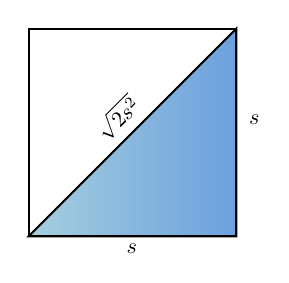
\begin{tikzpicture}[x=0.75pt,y=0.75pt,yscale=-1,xscale=1]
%uncomment if require: \path (0,300); %set diagram left start at 0, and has height of 300

%Shape: Square [id:dp7714270080777281] 
\draw   (11,11) -- (111,11) -- (111,111) -- (11,111) -- cycle ;
%Straight Lines [id:da32192438670599244] 
\draw    (11,111) -- (111,11) ;
%Shape: Right Triangle [id:dp44587122145691993] 
\path  [shading=_kd3za2b5b,_oobf9zdtu] (111,11) -- (11,111) -- (111,111) -- cycle ; % for fading 
 \draw   (111,11) -- (11,111) -- (111,111) -- cycle ; % for border 



% Text Node
\draw (58.6,58.6) node [anchor=south] [inner sep=0.75pt]  [rotate=-315,xscale=0.8,yscale=0.8]  {$\sqrt{2s^{2}}$};
% Text Node
\draw (57,113.4) node [anchor=north west][inner sep=0.75pt]  [xscale=0.8,yscale=0.8]  {$s$};
% Text Node
\draw (116,51.4) node [anchor=north west][inner sep=0.75pt]  [xscale=0.8,yscale=0.8]  {$s$};


\end{tikzpicture}
    \caption{A special case of the Pythagorean Theorem where each side is side length $s$ and the hypotenuse is $\sqrt{2s^2}$.}
    \label{fig:pythagSquare}
\end{figure}

\subsection{Distance between Points}

What is the distance between these two points?\index{distance using Pythagorean theorem}

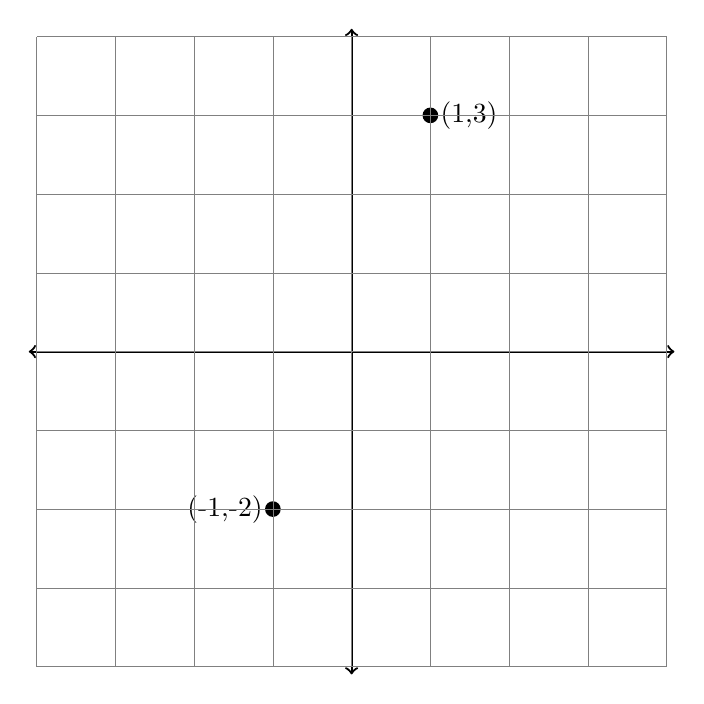
\begin{tikzpicture}
  % axis
  \draw[thick, <->] (0, -4.1) -- (0, 4.1);
  \draw[thick, <->] (-4.1, 0) -- (4.1, 0);
  \coordinate [circle, fill, inner sep=2pt] (a) at (-1,-2) ;
  \coordinate [circle, fill, inner sep=2pt] (b) at (1,3) ;
  \node [left] at (a) {(-1,-2)};
  \node [right] at (b) {(1,3)};
  % grid
  \draw[help lines, step = 1cm] (-4, -4) grid (4, 4);
  
\end{tikzpicture}

We can draw a right triangle and use the Pythagorean Theorem:

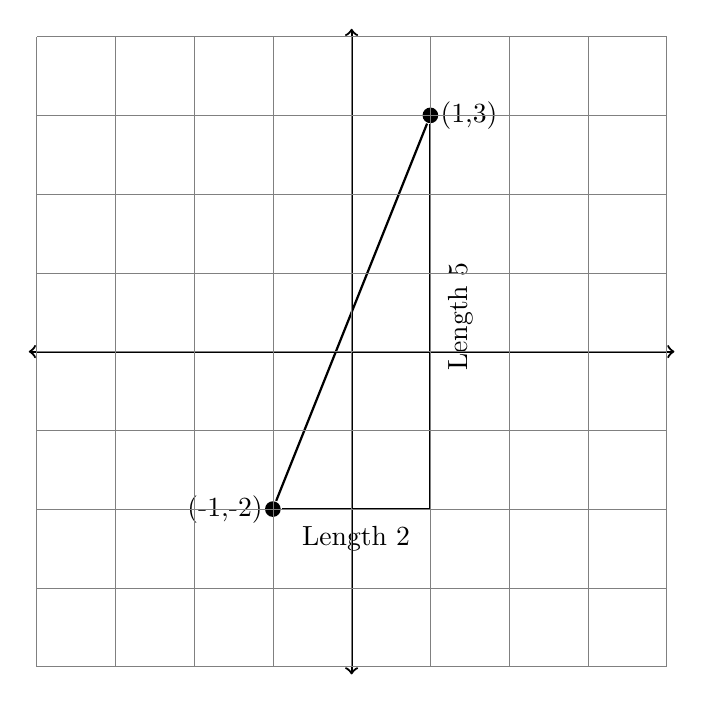
\begin{tikzpicture}
  % axis
  \draw[thick, <->] (0, -4.1) -- (0, 4.1);
  \draw[thick, <->] (-4.1, 0) -- (4.1, 0);
  \coordinate [circle, fill, inner sep=2pt] (a) at (-1,-2) ;
  \coordinate [circle, fill, inner sep=2pt] (b) at (1,3) ;
    \node [left] at (a) {(-1,-2)};
  \node [right] at (b) {(1,3)};
  \coordinate (c) at (1, -2);

  \draw [thick] (a) -- (b);
  \draw [thick] (a) -- node[outer sep = 3pt, below]{Length 2}(c);
  \draw [thick] (c) -- node[rotate=90, outer sep = 3pt, below]{Length 5}(b);
  \draw[help lines, step = 1cm] (-4, -4) grid (4, 4);
 
\end{tikzpicture}


The distance between the two points is $\sqrt{2^2 + 5^2} = \sqrt{29}
\approx 5.385165$. In other words, you square the change in $x$ and add it to
the square of the change in $y$. The distance is the square root of
that sum.

\subsection{Distance in 3 Dimensions}

What if the point is in three-dimensional space?  For example, you move 2
meters East, 8 meters North, and 4 meters up in the air. How far are
you from where you started?  You just square each, sum them, and take the square root:
$\sqrt{2^2 + 8^2 + 4^2} = \sqrt{84} = 2\sqrt{21} \approx 9.165$ meters.\index{distance!in 3 dimensions}

\begin{tikzpicture}
  \draw [thick, ->] (0,0,0) -- (9,0,0) node[outer sep = 1pt, right]{North} ; 
  \draw [thick, ->]  (0,0,0) -- (0,3,0) node[outer sep = 1pt, above]{Up} ; 
  \draw [thick, ->] (0,0,0) -- (0,0,4) node[outer sep = 1pt, below]{East} ; 

    \draw [dashed]  (8,0,0) -- node[outer sep = 1pt, right]{2}  (8,0,2); 

  \draw [dashed]  (0,0,2) -- node[outer sep = 1pt, below]{8} (8,0,2); 
  \draw [dashed]  (8,0,2) -- node[outer sep = 1pt, right]{4} (8,4,2); 
  \draw [thick]  (0,0,0) --  (8,4,2) node[circle, fill, inner sep=2pt]{}; 
  \node [left] at (5, 2.7, 1){$\sqrt{2^2 + 8^2 + 4^2} \approx 9.165$};

\end{tikzpicture}

This leads us to a formal definition of the \index{distance formula}distance formula:
\[
d = \sqrt{(x_2 - x_1)^2 + (y_2 - y_1)^2}
\]
Or in 3D space:
\[
d = \sqrt{(x_2 - x_1)^2 + (y_2 - y_1)^2 + (z_2 - z_1)^2}
\]


\section{Parallel and Perpendicular}
% vectors were not defined beforehand here
A \index{vector}\emph{vector} is an arrow: it has a length, called its \index{magnitude}\emph{magnitude}, and a direction. Velocity, force, and displacement are all vectors.

Two vectors are \emph{parallel}\index{parallel} if they point in the same direction or in exactly opposite directions; their lengths do not matter. Two cars driving north are moving in parallel, and so are a car driving north and a car driving south.

\begin{center}
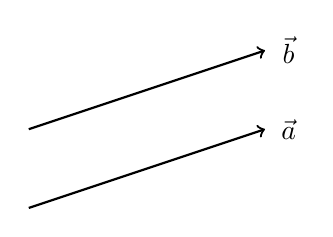
\begin{tikzpicture}[scale=1]
    \draw[thick,->] (0,0) -- (3,1);
    \draw[thick,->] (0,1) -- (3,2);
    \node at (3.3,1) {$\vec{a}$};
    \node at (3.3,2) {$\vec{b}$};
\end{tikzpicture}
\end{center}

Two vectors are \emph{perpendicular}\index{perpendicular} if they meet at a right angle, like the $x$- and $y$-axes, or the edges of a sheet of paper.

\begin{center}
\begin{tikzpicture}[scale=.5]
    % Draw x and y axes
    \draw[->] (-5,0) -- (5,0) node[right] {$x$};
    \draw[->] (0,-5) -- (0,5) node[above] {$y$};
    % Optional: mark the origin
    \node at (0,0) [below left] {O};
\end{tikzpicture}
\end{center}

Perpendicular vectors have a handy property: their \index{dot product}\emph{dot product} is zero. You will learn the dot product in the vectors chapter, and it will give you a quick test for whether two vectors are perpendicular. In the next chapter, you will graph parallel and perpendicular lines and find their equations.

%FIXME would a section on perpendicular bisectors, alternate interior/exterior angles, and transversals fit here?
